\subsection{Results}
To get an idea of how many features each image descriptor produces, we will begin this section by taking a look at three image pairs where each image descriptor have been run. The found features can be seen in \autoref{noFeatures}, and only shows correct correspondences. By manual inspection, it can also be reported that in general (when not constrained) SIFT and SURF produces more matches than ORB.

\begin{figure}[h]
	\centering
	\begin{subfigure}{0.8\linewidth}
		\centering
		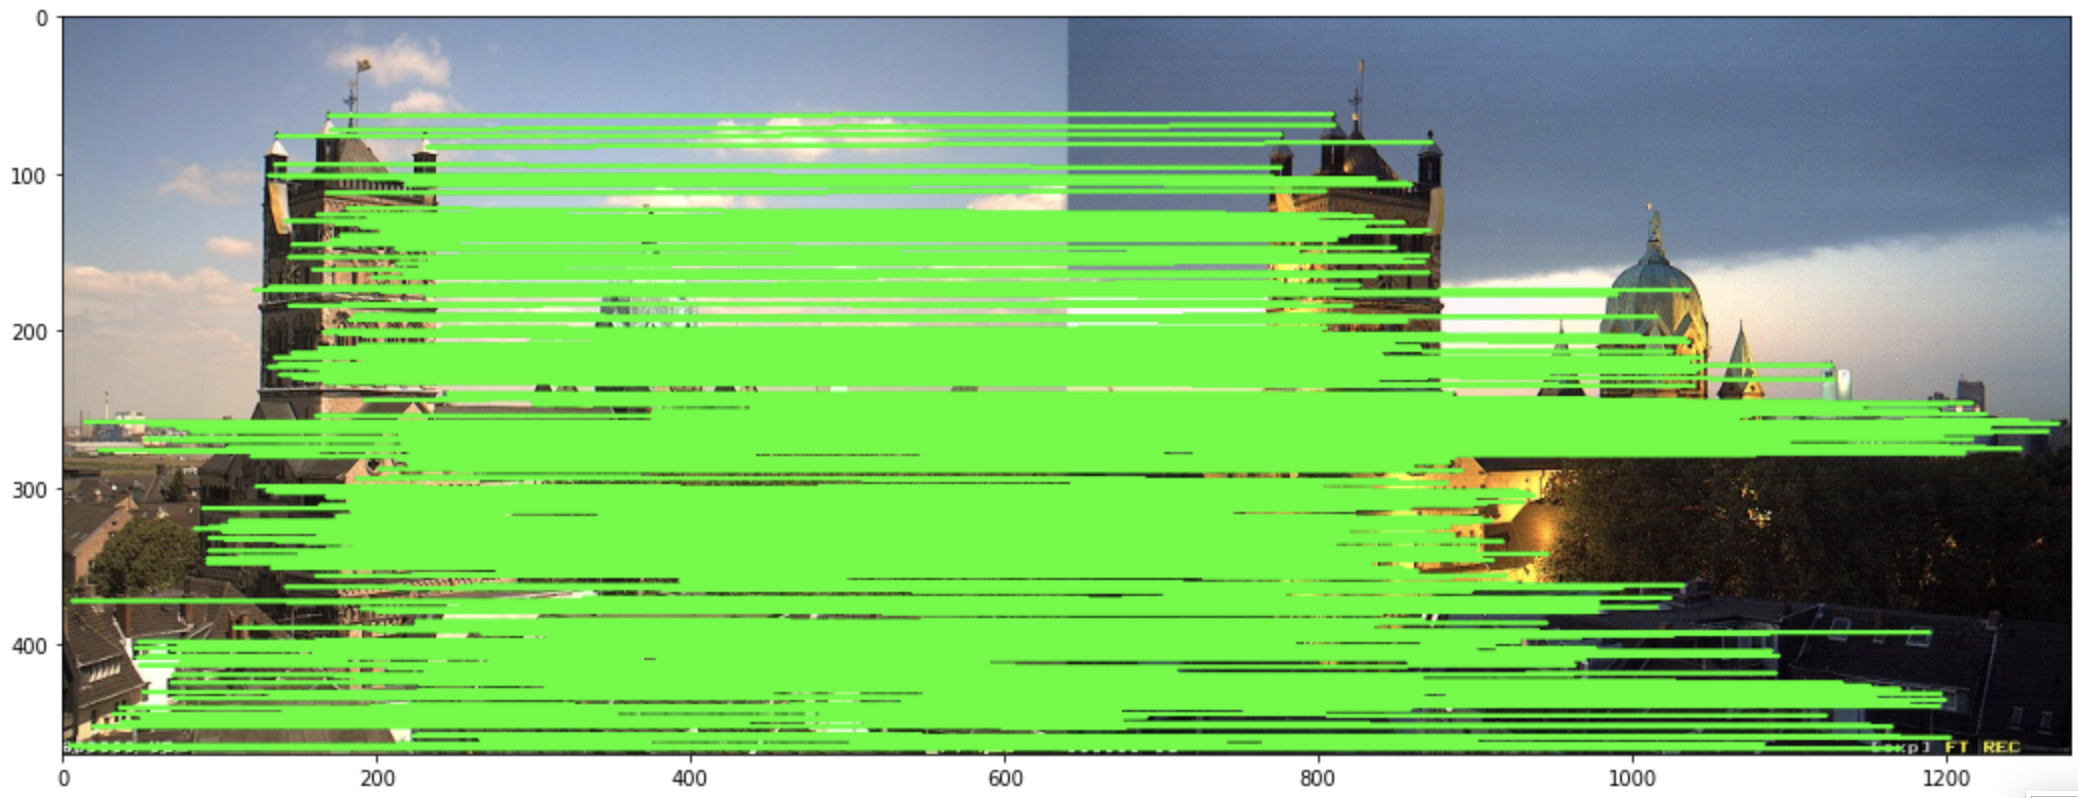
\includegraphics[width=\linewidth]{Materials/SIFTMatches}
		\caption{The detected SIFT features.}
	\end{subfigure}
	\\
	\begin{subfigure}{0.8\linewidth}
		\centering
		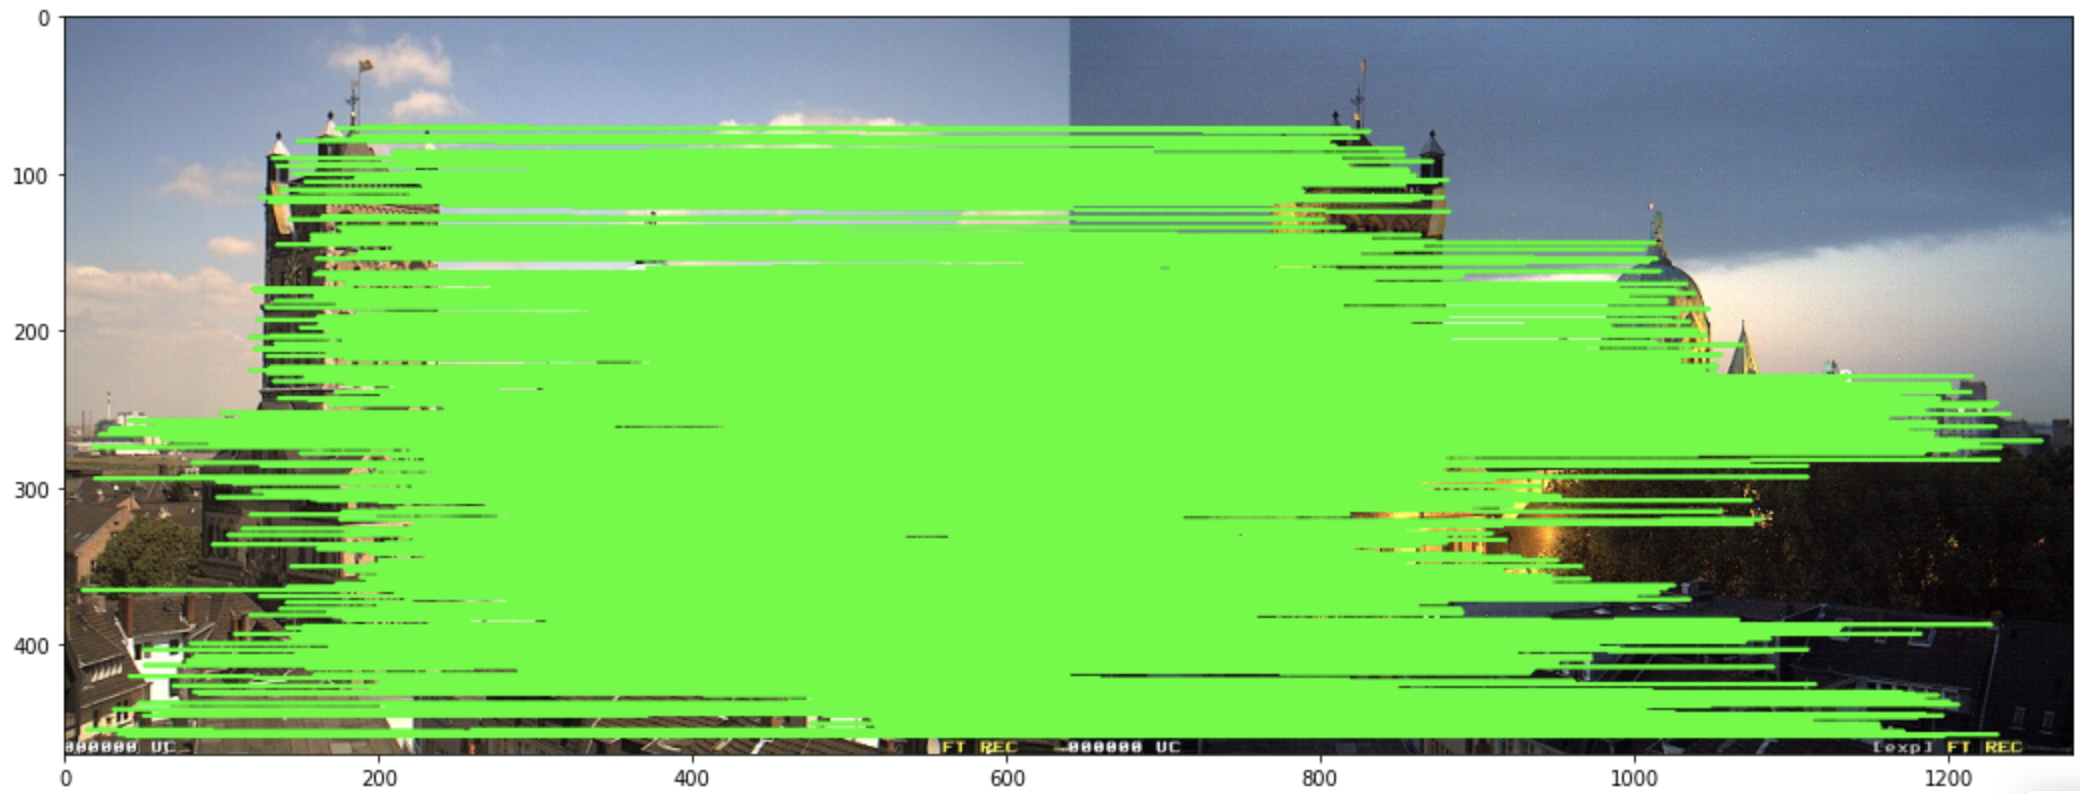
\includegraphics[width=\linewidth]{Materials/SURFMatches}
		\caption{The detected SURF features.}
	\end{subfigure}
	\\
	\begin{subfigure}{0.8\linewidth}
		\centering
		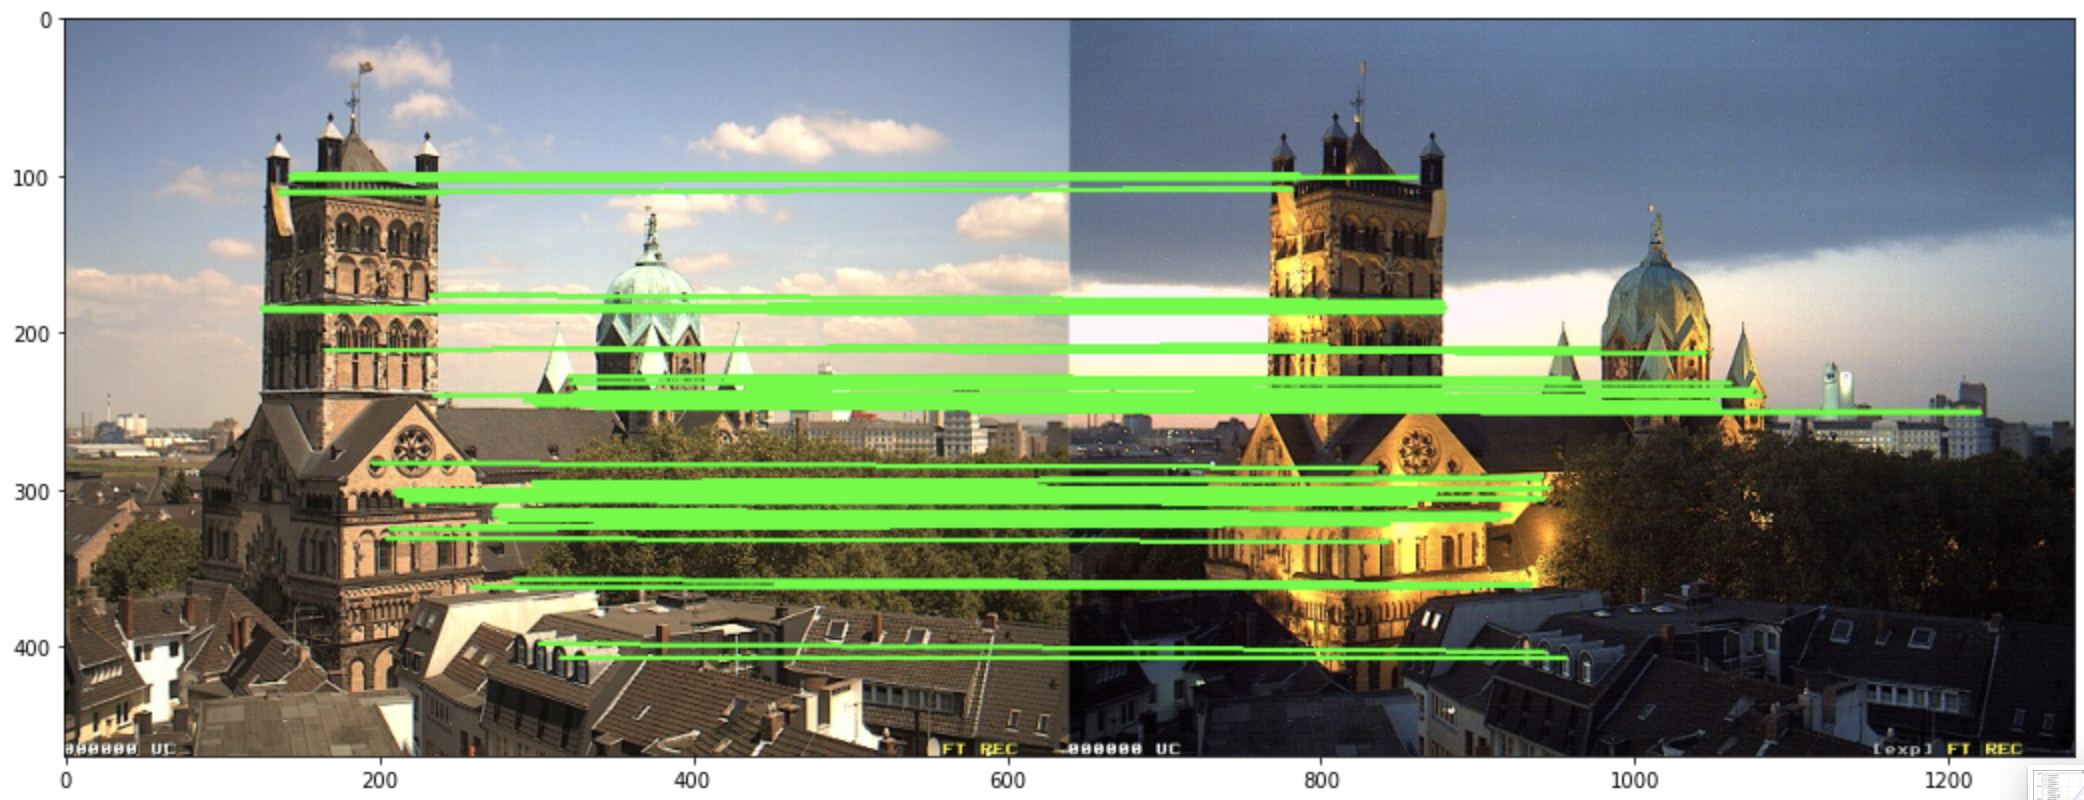
\includegraphics[width=\linewidth]{Materials/ORBMatches}
		\caption{The detected ORB features.}
	\end{subfigure}
	\caption{Each image descriptor run on the same image pair to give an indication of how many features each finds.}
	\label{noFeatures}
\end{figure}

\begin{table}[h]
	\centering
	\begin{tabular}{|c||ccc||ccc||c|}
		\hline
		& \multicolumn{3}{c||}{Homography estimation}                           & \multicolumn{3}{c||}{Mean localization error}                          & NN mean average precision \\ \hline
		& \multicolumn{1}{c|}{eps = 1} & \multicolumn{1}{c|}{eps = 3} & eps = 5 & \multicolumn{1}{c|}{eps = 1} & \multicolumn{1}{c|}{eps = 3} & eps = 5 &                           \\ \hline
		SIFT & \multicolumn{1}{c|}{0.34}   & \multicolumn{1}{c|}{0.61}    & 0.71    & \multicolumn{1}{c|}{0.56}    & \multicolumn{1}{c|}{1.46}    & 2.41    & 0.72                      \\ \hline
		ORB  & \multicolumn{1}{c|}{0.05}   & \multicolumn{1}{c|}{0.21}    & 0.31    & \multicolumn{1}{c|}{0.54}    & \multicolumn{1}{c|}{1.54}    & 2.41    & 0.73                      \\ \hline
		SURF & \multicolumn{1}{c|}{0.29}   & \multicolumn{1}{c|}{0.53}    & 0.66    & \multicolumn{1}{c|}{0.56}    & \multicolumn{1}{c|}{1.48}    & 2.27    & 0.50                      \\ \hline
	\end{tabular}
	\caption{Results of the experiments.}
	\label{results}
\end{table}
As seen, SIFT finds about as many features as SURF whereas ORB finds a considerable amount less.\\
In \autoref{results} we see the results of the experiments conducted. When comparing SIFT and ORB we see their ability to estimate correct homographies varies greatly. ORB estimates as many correctly homographies when epsilon is 5 as SIFT does when epsilon is 1, that is, SIFT is much more accurate when estimating homographies. SURF lies in between the two, performing closer to SIFT than ORB. However, when we compare the mean localization error SIFT, SURF and ORB obtain similar errors. This means their ability to choose the same places in the image pairs are equivalent. However, looking at the actual errors, we see the error is about halfway between the minimum and maximum possible which means we are fairly far away from the actual location we were looking for. When it comes to nearest neighbour mean average precision SIFT and ORB performs similar and fairly well, whereas SURF performs quite poorly.